\documentclass[a4paper,11pt,german,notitlepage]{report}
\usepackage{xcolor}
\usepackage{tabularx}
\usepackage{dclecture}
\usepackage{qrcode}
\usepackage{awesomebox}
\usepackage{circuitikz}
\usepackage[style=german, german=swiss]{csquotes}
\def\farbe{darkgray} %Hier Farbe definieren
\addbibresource{refs.bib}

\ctikzset{
    logic ports=ieee,
    logic ports/scale=0.8,
    logic ports/fill=lightgray
}

\usetikzlibrary{arrows,shapes.gates.logic.US,shapes.gates.logic.IEC,calc,positioning}

\graphicspath{{img/}}

% Extract Exercises

%\usepackage[active, generate=trigonometry_exercises, extract-env={ex}]{extract}
%\begin{extract}
%\usepackage{xcolor}
%\def\farbe{teal}
%\usepackage{dcexercisesnogrid}
%\exercisetrue
%\end{extract}


%%% Fancy Header and Footer
\renewcommand{\headrule}{\vbox to 0pt{\hbox to\headwidth{\color{\farbe}\rule{\headwidth}{1pt}}\vss}}
\pagestyle{fancy} %eigener Seitenstil
\fancyhf{} %alle Kopf- und Fu§zeilenfelder bereinigen
\fancyhead[C]{Informatik - Gymnasium 1. Klasse - Algorithmen Projekt - Food Delivery Dienst} %Kopfzeile mitte
%\fancyhead[R]{\includegraphics[width=0.2cm]{x.png}}

\fancyfoot[C]{\thepage}

%\rfoot{\setlength{\unitlength}{1mm}
%\begin{picture}(0,0)
%\put(5,0){\includegraphics{pic\thepage.ps}}
%\end{picture}}


\parskip=.1cm
\parindent=0cm
\linespread{1.5}



\begin{document}

\section*{Beschreibung}
In diesem Projekt nehmen Sie die Rolle der imaginären Firma Food Sprint ein, welche Essen liefert.
\begin{figure}[h!]
    \centering
    
\includegraphics[height=3cm]{logo.png}  
\end{figure}
Ihr Ziel ist es für Ihren Fahrer mögslicht effiziente Routen zu planen, damit dieser das Essen liefern kann, während es noch warm ist.
Der Einfachheit halber verwenden wir nicht eine Stadtkarte, sondern ein simples Koordinatiensystem um zu navigieren.
Zur Notation verwenden wir $x$ und $y$.\\
$x =$ Spalte (von links nach rechts): $0, 1, 2, 3, 4$;
$y =$ Reihe (von unten nach oben): $0, 1, 2, 3, 4$;
Sie wissen bereits im Voraus, wohin die Lieferungen gehen müssen (dies wird jeweils zufällig generiert).
Und zwar haben Sie zu jeder Lieferung die genauen Koordinaten $(x,y)$.
Sie müssen immer genau drei Lieferungen ausliefern.
\begin{figure}[h!]
    \centering
    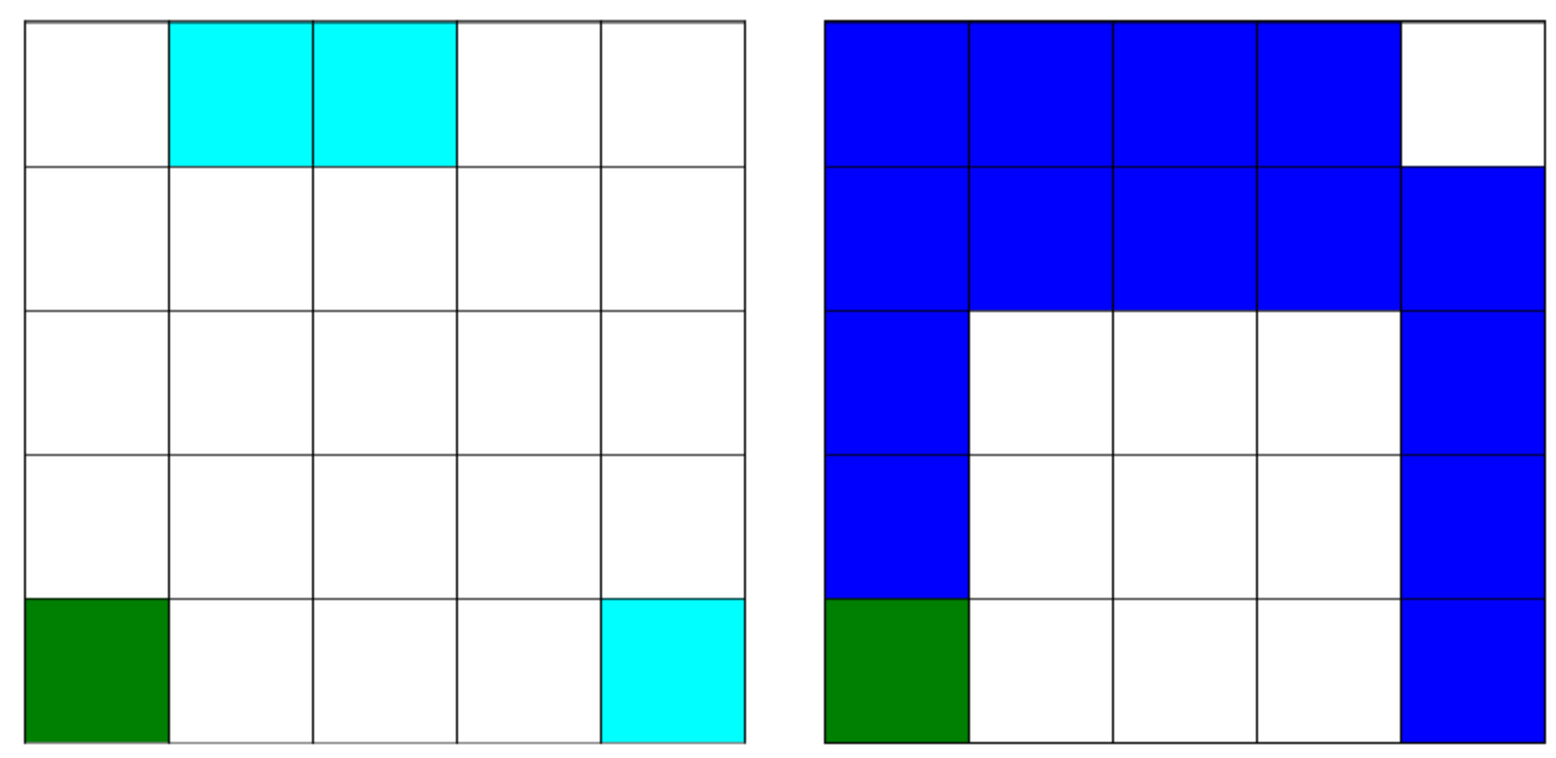
\includegraphics[height=4.5cm]{food_service.png}  
    \caption{Screenshot von WebTigerJython. Eine mögliche Route, um das Essen zu liefern. War das wohl der schnellste Weg?}
\end{figure}
In diesem Projekt beginnen Sie bereits mit einer implementierten Suche in der Codevorlage.
Diese Suche ist jedoch nicht optimal.

\section*{Regeln}
\begin{description}
    \item[Ziel:] Das Essen soll so effizient wie möglich ausgeliefert werden. Das Ziel ist erreicht, wenn Sie mit der Suche alle Kunden gefunden haben und das Essen geliefert ist.
    \item[Züge:] Ihr Fahrer kann sich horizontal, vertikal und diagonal jeweils ein Feld bewegen.
\end{description}
\section*{Farbencodes}
\begin{description}
    \item[Grün] Die Station des Lieferservice, die Suche beginnt hier. Sie liegt immer bei $(0,0)$
    \item[Cyan] Ort der Bestellung, hier können Sie das Essen abliefern. 
    \item[Weiss] Eine Strasse in der Stadt.
\end{description}


\section*{Aufgabe}
Hier werden zusätzliche Aufgaben beschrieben, welche spezifisch für Ihr Projekt sind.
Die Aufgaben sind in zwei Gruppen unterzeilt: Pflichtaufgaben und optionale Aufgaben.
Die Pflichtaufgaben sollen am Ende des Projektes beantwortet sein.
Die optionalen Aufgaben dienen dazu, sich weiter im Thema zu vertiefen.
Diese Aufgaben sind Vorschläge. Sie dürfen auch eigene Fragestellungen vertiefen.
Deklarieren Sie Ihre Fragestellungen klar im Projektbericht.
Für alle Projekt gilt natürlich, dass Sie zuerst die allgemeine Aufgabenstellung und den Code (falls vorhanden) verstehen sollten, bevor Sie die untenstehen Aufgaben bearbeiten.
\subsection*{Pflichtaufgaben}
\begin{itemize}
    \item In der Vorlage ist bereits die Tiefensuche Implementiert. Was fällt auf?
    \item Versuchen Sie für diese Problem als erstes Die Breitensuche zu implementieren. Was für Probleme ergeben sich? Ist die Lösung optimal?
    \item Reflektieren Sie, welche Regeln bezüglich Pruning für Ihr spezifisches Problem sinnvoll sind und welche nicht. Was für eine Auswirkung auf mögliche Lösungen haben die verschiedenen Pruningstrategien?
    \item Schreiben Sie ein Programm (oder verbessern Sie das existierende), welches jeweils eine optimale Lösung für Ihr Problem findet. Um dies Umzusetzen, überlegen Sie sich Sie sich eine Heuristik, welche die Koordinaten der Lieferorte verwendet.
\end{itemize}
\subsection*{Optionale Aufgaben}
\begin{itemize}
    \item Was passiert, wenn Sie die Konfiguration ändern, also beispielsweise die Breite und die Höhe verdoppeln und statt 3, 5 Lieferungen durchführen müssen? Können Sie sich eine Heuristik, welche auch bei sehr grossen Problemen zu einer effizienten Suche führt?
    \item (Sehr schwierig) Recherchieren Sie den Fachbegriff \textit{Landmark Heuristik Search}. Überlegen Sie, wie Sie diese Technik in diesem Problem anwenden könnten.
\end{itemize}

\end{document}  
